\documentclass[11pt]{article}
\usepackage[textwidth=18.0cm, textheight=23.0cm, top=2.0cm]{geometry}
\usepackage{pst-all}
\usepackage{amssymb}
\usepackage{tikz}
\usepackage{underscore}\begin{document}
\pagestyle{empty}


ClassName: \underline{\textbf{Class_06.2bp-14}}
\par
BinSize: \underline{\textbf{300 × 300}}
\par
ReduceSize: \underline{\textbf{300 × 300}}
\par
TypeNum: \underline{\textbf{40}}
\par
Num: \underline{\textbf{40}}
\par
OutS: \underline{\textbf{180000}}
\par
InS: \underline{\textbf{119011}}
\par
Rate: \underline{\textbf{0.661}}
\par
UB: \underline{\textbf{2}}
\par
LB0: \underline{\textbf{2}}
\par
LB: \underline{\textbf{2}}
\par
LBWithCut: \underline{\textbf{2}}
\par
NodeCut: \underline{\textbf{0}}
\par
ExtendedNodeCnt: \underline{\textbf{1}}
\par
GenNodeCnt: \underline{\textbf{1}}
\par
PrimalNode: \underline{\textbf{0}}
\par
ColumnCount: \underline{\textbf{2}}
\par
TotalCutCount: \underline{\textbf{0}}
\par
RootCutCount: \underline{\textbf{0}}
\par
LPSolverCnt: \underline{\textbf{1}}
\par
PricingSolverCnt: \underline{\textbf{0}}
\par
BranchAndBoundNum: \underline{\textbf{1}}
\par
isOpt: \underline{\textbf{true}}
\par
TimeOnInitSolution: \underline{\textbf{600.000 s}}
\par
TimeOnPrimal: \underline{\textbf{0.000 s}}
\par
TimeOnPricing: \underline{\textbf{0.000 s}}
\par
TimeOnRmp: \underline{\textbf{0.063 s}}
\par
TotalTime: \underline{\textbf{600.344 s}}
\par
\newpage


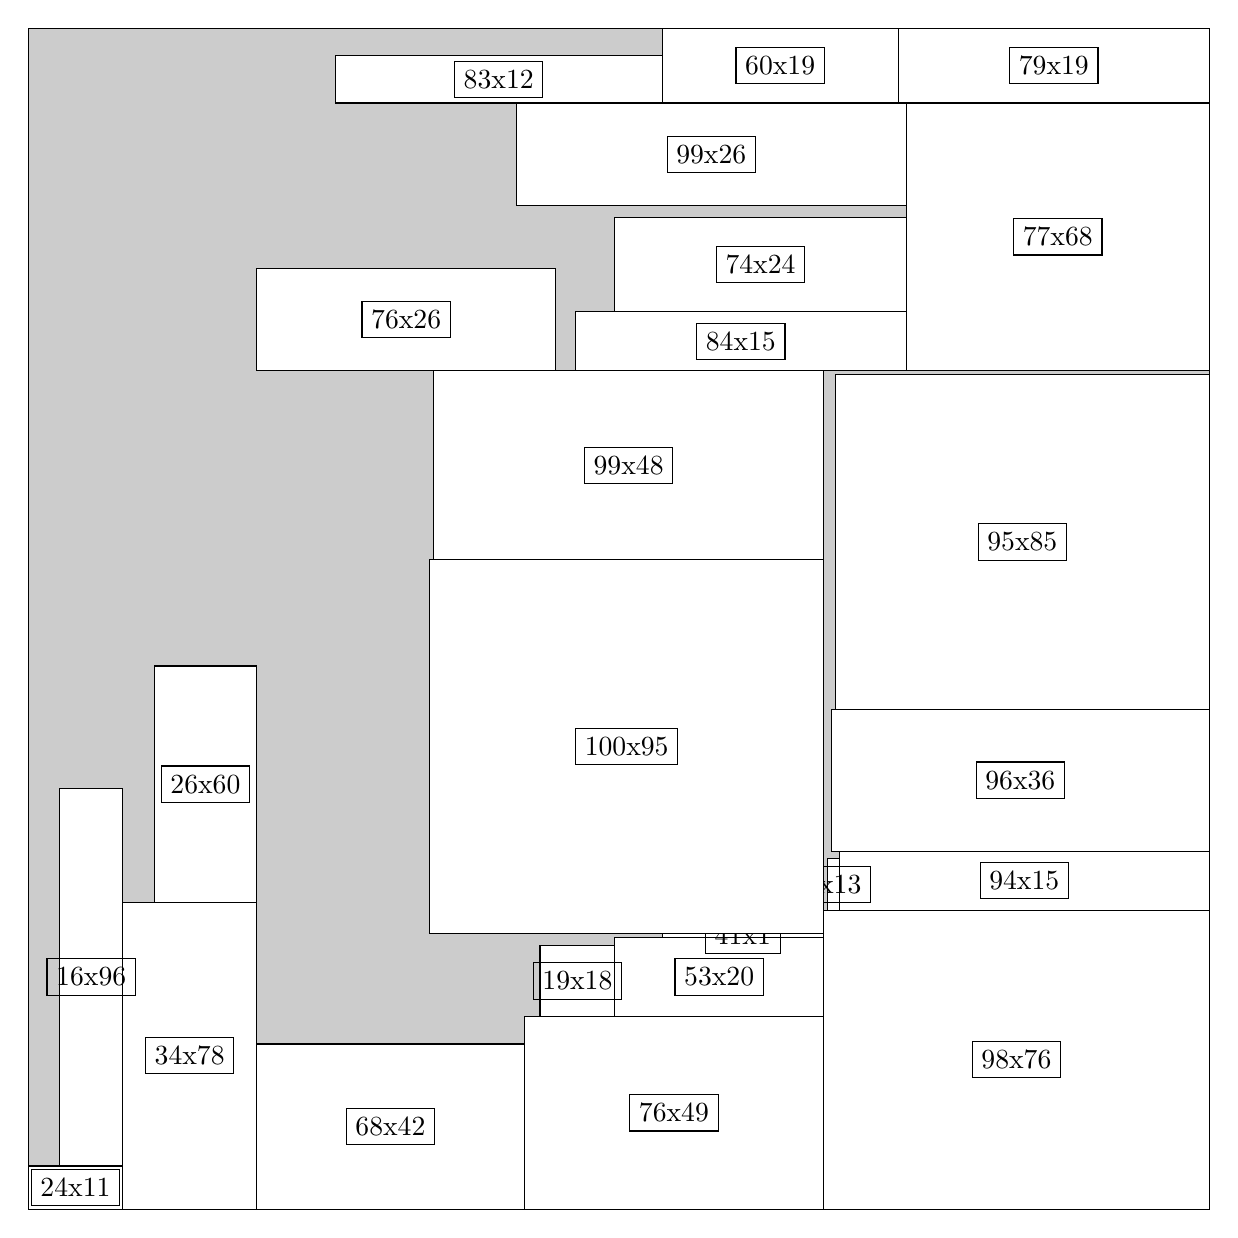
\begin{tikzpicture}[shorten >=1pt,scale=1.0,every node/.style={scale=1.0},->]
\tikzstyle{vertex}=[circle,fill=black!25,minimum size=14pt,inner sep=0pt]
\filldraw[fill=gray!40!white, draw=black] (0,0) rectangle (15.0,15.0);
\foreach \name/\x/\y/\w/\h in {98x76/10.100000000000001/0.0/4.9/3.8000000000000003,94x15/10.3/3.8000000000000003/4.7/0.75,3x13/10.15/3.8000000000000003/0.15000000000000002/0.65,96x36/10.200000000000001/4.55/4.800000000000001/1.8,95x85/10.25/6.3500000000000005/4.75/4.25,76x49/6.300000000000001/0.0/3.8000000000000003/2.45,53x20/7.45/2.45/2.6500000000000004/1.0,41x1/8.05/3.45/2.0500000000000003/0.05,19x18/6.5/2.45/0.9500000000000001/0.9,68x42/2.9000000000000004/0.0/3.4000000000000004/2.1,100x95/5.1000000000000005/3.5/5.0/4.75,99x48/5.15/8.25/4.95/2.4000000000000004,77x68/11.15/10.65/3.85/3.4000000000000004,84x15/6.95/10.65/4.2/0.75,74x24/7.45/11.4/3.7/1.2000000000000002,76x26/2.9000000000000004/10.65/3.8000000000000003/1.3,99x26/6.2/12.75/4.95/1.3,34x78/1.2000000000000002/0.0/1.7000000000000002/3.9000000000000004,26x60/1.6/3.9000000000000004/1.3/3.0,79x19/11.05/14.05/3.95/0.9500000000000001,60x19/8.05/14.05/3.0/0.9500000000000001,83x12/3.9000000000000004/14.05/4.15/0.6000000000000001,24x11/0.0/0.0/1.2000000000000002/0.55,16x96/0.4/0.55/0.8/4.800000000000001}
\filldraw[fill=white!40!white, draw=black] (\x,\y) rectangle node[draw] (\name) {\name} ++(\w,\h);
\end{tikzpicture}


w =98 , h =76 , x =202 , y =0 , v =7448
\par
w =94 , h =15 , x =206 , y =76 , v =1410
\par
w =3 , h =13 , x =203 , y =76 , v =39
\par
w =96 , h =36 , x =204 , y =91 , v =3456
\par
w =95 , h =85 , x =205 , y =127 , v =8075
\par
w =76 , h =49 , x =126 , y =0 , v =3724
\par
w =53 , h =20 , x =149 , y =49 , v =1060
\par
w =41 , h =1 , x =161 , y =69 , v =41
\par
w =19 , h =18 , x =130 , y =49 , v =342
\par
w =68 , h =42 , x =58 , y =0 , v =2856
\par
w =100 , h =95 , x =102 , y =70 , v =9500
\par
w =99 , h =48 , x =103 , y =165 , v =4752
\par
w =77 , h =68 , x =223 , y =213 , v =5236
\par
w =84 , h =15 , x =139 , y =213 , v =1260
\par
w =74 , h =24 , x =149 , y =228 , v =1776
\par
w =76 , h =26 , x =58 , y =213 , v =1976
\par
w =99 , h =26 , x =124 , y =255 , v =2574
\par
w =34 , h =78 , x =24 , y =0 , v =2652
\par
w =26 , h =60 , x =32 , y =78 , v =1560
\par
w =79 , h =19 , x =221 , y =281 , v =1501
\par
w =60 , h =19 , x =161 , y =281 , v =1140
\par
w =83 , h =12 , x =78 , y =281 , v =996
\par
w =24 , h =11 , x =0 , y =0 , v =264
\par
w =16 , h =96 , x =8 , y =11 , v =1536
\par
\newpage


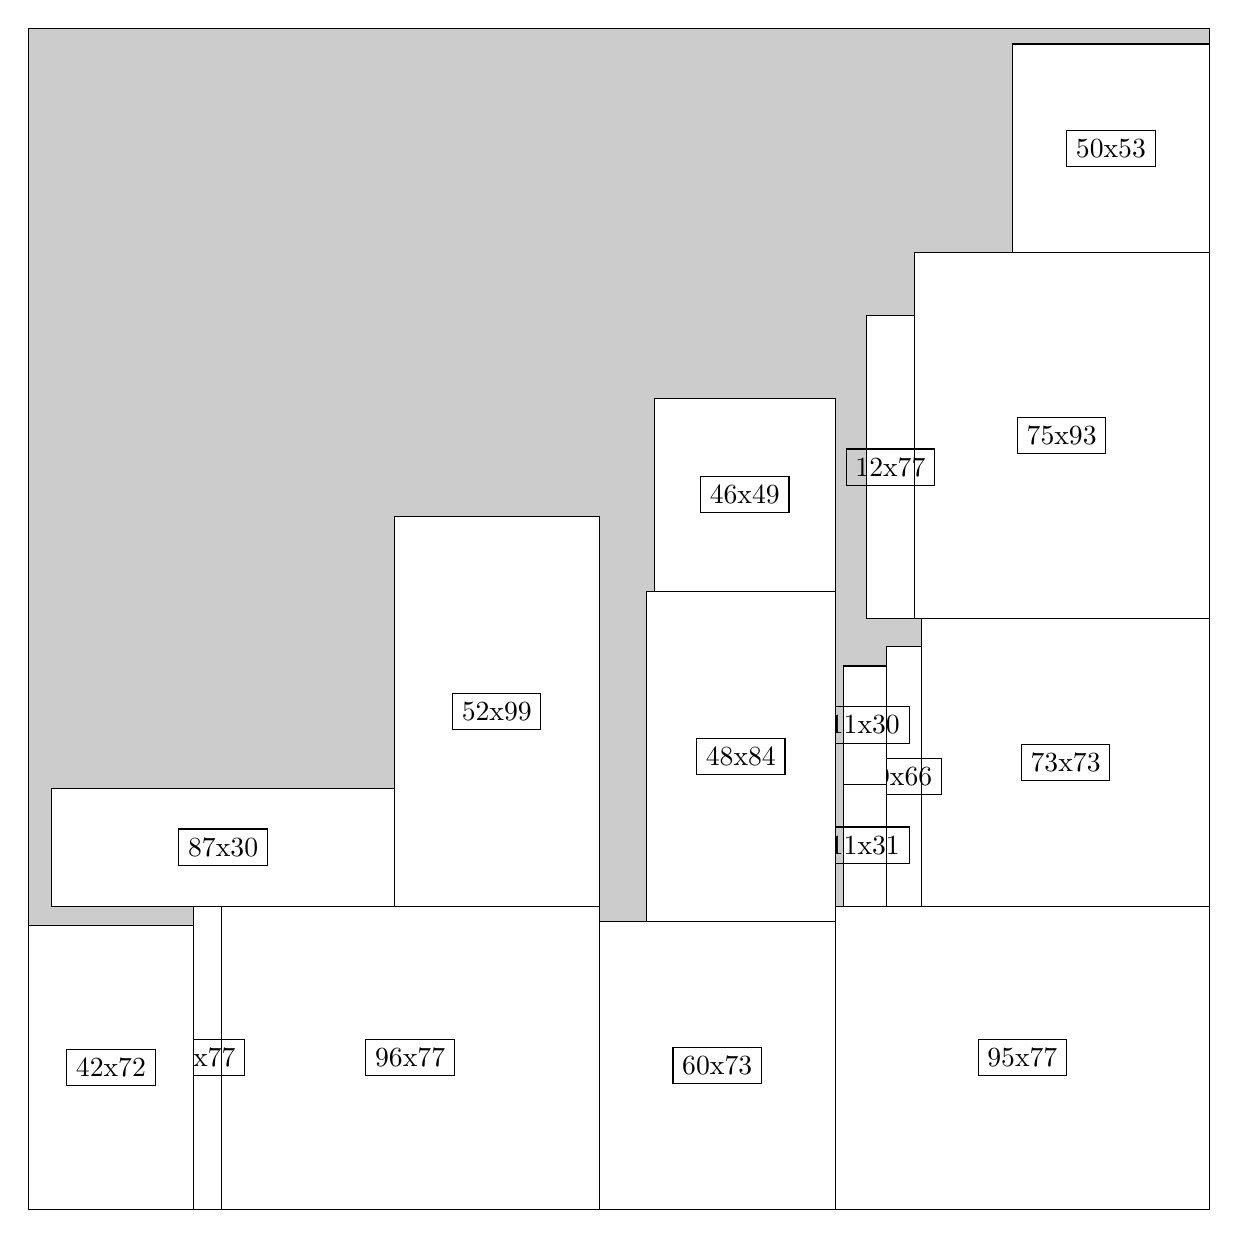
\begin{tikzpicture}[shorten >=1pt,scale=1.0,every node/.style={scale=1.0},->]
\tikzstyle{vertex}=[circle,fill=black!25,minimum size=14pt,inner sep=0pt]
\filldraw[fill=gray!40!white, draw=black] (0,0) rectangle (15.0,15.0);
\foreach \name/\x/\y/\w/\h in {95x77/10.25/0.0/4.75/3.85,73x73/11.350000000000001/3.85/3.6500000000000004/3.6500000000000004,9x66/10.9/3.85/0.45/3.3000000000000003,11x31/10.350000000000001/3.85/0.55/1.55,11x30/10.350000000000001/5.4/0.55/1.5,75x93/11.25/7.5/3.75/4.65,12x77/10.65/7.5/0.6000000000000001/3.85,50x53/12.5/12.15/2.5/2.6500000000000004,60x73/7.25/0.0/3.0/3.6500000000000004,48x84/7.8500000000000005/3.6500000000000004/2.4000000000000004/4.2,46x49/7.95/7.8500000000000005/2.3000000000000003/2.45,96x77/2.45/0.0/4.800000000000001/3.85,7x77/2.1/0.0/0.35000000000000003/3.85,42x72/0.0/0.0/2.1/3.6,52x99/4.65/3.85/2.6/4.95,87x30/0.30000000000000004/3.85/4.3500000000000005/1.5}
\filldraw[fill=white!40!white, draw=black] (\x,\y) rectangle node[draw] (\name) {\name} ++(\w,\h);
\end{tikzpicture}


w =95 , h =77 , x =205 , y =0 , v =7315
\par
w =73 , h =73 , x =227 , y =77 , v =5329
\par
w =9 , h =66 , x =218 , y =77 , v =594
\par
w =11 , h =31 , x =207 , y =77 , v =341
\par
w =11 , h =30 , x =207 , y =108 , v =330
\par
w =75 , h =93 , x =225 , y =150 , v =6975
\par
w =12 , h =77 , x =213 , y =150 , v =924
\par
w =50 , h =53 , x =250 , y =243 , v =2650
\par
w =60 , h =73 , x =145 , y =0 , v =4380
\par
w =48 , h =84 , x =157 , y =73 , v =4032
\par
w =46 , h =49 , x =159 , y =157 , v =2254
\par
w =96 , h =77 , x =49 , y =0 , v =7392
\par
w =7 , h =77 , x =42 , y =0 , v =539
\par
w =42 , h =72 , x =0 , y =0 , v =3024
\par
w =52 , h =99 , x =93 , y =77 , v =5148
\par
w =87 , h =30 , x =6 , y =77 , v =2610
\par
\newpage


\end{document}